% Jacob Neumann

% DOCUMENT CLASS AND PACKAGE USE
    \documentclass[aspectratio=169, handout]{beamer}

    % Establish the colorlambda boolean, to control whether the lambda is solid color (true), or the same as the picture (false)
    \newif\ifcolorlambda
    \colorlambdafalse % DEFAULT: false

    % Use auxcolor for syntax highlighting
    \newif\ifuseaux
    \useauxfalse % DEFAULT: false

    % Color settings
    \useauxtrue

    \newcommand{\auxColor}{039c1a}     % the color of note boxes and stuff
    \newcommand{\presentColor}{E45535} % the primary color of the slide borders
    \newcommand{\bgColor}{e3f3ff}      % the color of the background of the slide
    \newcommand{\darkBg}{8b98ad}
    \newcommand{\lambdaColor}{\auxColor}

    \colorlambdatrue

    \usepackage{comment} % comment blocks
    \usepackage{soul} % strikethrough
    \usepackage{listings} % code
    \usepackage{makecell}
    \usepackage{mathtools} % for \mathrlap


    \setbeamertemplate{itemize items}[circle]
    % \setbeameroption{show notes on second screen=right}

    \usepackage{lectureSlides}
    %%%%%%%%%%%%%%%%%%%%%%%%%%%%%%%%%%%%%%%%%| <----- Don't make the title any longer than this
    \title{Polymorphism} % TODO
    \subtitle{Awesome slides with an awesome subtitle} % TODO
    \date{01 January 2020} % TODO
    \author{Brandon Wu} % TODO

    \graphicspath{ {./img/} }
    % DONT FORGET TO PUT [fragile] on frames with codeblocks, specs, etc.
        %\begin{frame}[fragile]
        %\begin{codeblock}
        %fun fact 0 = 1
        %  | fact n = n * fact(n-1)
        %\end{codeblock}
        %\end{frame}

    % INCLUDING codefile:
        % 1. In some file under code/NN (where NN is the lecture id num), include:
    %       (* FRAGMENT KK *)
    %           <CONTENT>
    %       (* END KK *)

    %    Remember to not put anything on the same line as the FRAGMENT or END comment, as that won't be included. KK here is some (not-zero-padded) integer. Note that you MUST have fragments 0,1,...,KK-1 defined in this manner in order for fragment KK to be properly extracted.
        %  2. On the slide where you want code fragment K
                % \smlFrag[color]{KK}
        %     where 'color' is some color string (defaults to 'white'. Don't use presentColor.
    %  3. If you want to offset the line numbers (e.g. have them start at line 5 instead of 1), use
                % \smlFragOffset[color]{KK}{5}

\begin{document}

% Make it so ./mkWeb works correctly
\ifweb
    \renewcommand{\pause}{}
\fi

\setbeamertemplate{itemize items}[circle]

% SOLID COLOR TITLE (see SETTINGS.sty)
{
\begin{frame}[plain]
    \colorlambdatrue
    \titlepage
\end{frame}
}

\menti{2165 5174}

\begin{frame}[fragile]
  \frametitle{Lesson Plan}

  \tableofcontents
\end{frame}

\begin{frame}[fragile]
  \frametitle{Last time}

  Last time, we discussed the \term{tree method} and how it can be used to
  solve more difficult recurrences, that make multiple recursive calls.

  \pause
  \vspace{\fill}

  We also learned how to analyze complexity of a function on trees via
  depth as opposed to the number of nodes. We saw that this obtained
  different bounds, but through reasoning about the relationship between
  nodes and depth, ultimately came out to be the same .

  \pause
  \vspace{\fill}

  We then explored sorting, and wrote a terse implementation of \term{merge sort},
  and then analyzed its work and span.
\end{frame}

\sectionSlide{1}{Type Inference}

\begin{frame}[fragile]
  \frametitle{An Overflow of \code{int}}

  You may have noticed that we've been using \code{int}s all over the place.

  \pause
  \vspace{\fill}

  We've so far dealt with lists of ints, trees of ints, and sorting ints. We've
  been focusing on things of type \code{int} quite a bit, but we haven't had to!
  We might be interested in data structures which hold things which are not
  just integers, for instance.

  \pause
  \vspace{\fill}

  If we did that, however, we would need to redo every lecture that we've done
  up to this point, because everything we've discovered has only been for the type
  \code{int}! If only there were some way of doing things in a generic way, for
  any type.
\end{frame}

\begin{frame}[fragile]
  \frametitle{The \code{length} function}

  Recall the \code{length} function we defined long ago:

  \pause
  \begin{codeblock}
    fun length ([] : int list) : int = 0
      | length (x::xs) = 1 + length xs
  \end{codeblock}

  \pause
  \vspace{\fill}

  This only works on lists of type \code{int}, but there's no reason for it
  to! We could have easily written it as:

  \pause
  \begin{codeblock}
    fun length ([] : int list) : int = 0
      | length (_::xs) = 1 + length xs
  \end{codeblock}

  and never inspected any specific element of the list at all.
\end{frame}

\begin{frame}[fragile]
  \frametitle{Type Annotations}

  \tgs

  We have been type annotating our code the entire semester. In keeping with
  our Big Idea that \term{Types Guide Structure}, we want to make sure that
  the structure of our code is easily described via types.

  \pause
  \vspace{\fill}

  This is often a lot of work, however! We know that SML is able to automatically
  determine whether an expression is ill-typed -- that is, if there types are
  used in a contradictory way. Is SML also able to determine the type of programs
  automatically?

  \pause
  \vspace{\fill}

  The answer: \textbf{It is!}
\end{frame}

\begin{frame}[fragile]
  \frametitle{Type Inference}

  SML performs \term{type inference}, which is the automatic derivation of
  types for all expressions. When this process fails, the program is rejected
  as ill-typed.\footnote{
    You might say that the SML type system has type \code{expression -> typ option}.
  }

  \pause
  \vspace{\fill}

  The type inference algorithm is basically a straightforward recursive
  algorithm on an expression. When we encounter a function that we know to have
  a certain type, we assume that it type-checks, and then recurse to see
  if there are any contradictions.
\end{frame}

\begin{frame}[fragile]
  \frametitle{Type Inference: An Example}

  Suppose we are inferring a type for the expression \code{2 + 3}.

  \pause
  \vspace{\fill}

  Since this is just the application of a function \code{+ : int * int -> int},
  we assume it has type \code{int}.

  \pause
  \vspace{\fill}

  We then check whether \code{2 : int}, which it does, so no contradiction.

  \pause
  \vspace{\fill}

  We then check whether \code{3 : int}, which it does, so no contradiction.

  \pause
  \vspace{\fill}

  So \code{2 + 3} type-checks, and additionally, has type \code{int}.
\end{frame}

\begin{frame}[fragile]
  \frametitle{Type Inference: Functions}

  It's more interesting when we get into examples with functions!

  \pause
  \vspace{\fill}

  When a function accepts an argument, it has a yet-unknown type. When
  inferring the type of such a variable, the type inference algorithm must
  use the context of \textit{how the variable is used} to determine the
  variable's type.

  \pause
  \vspace{\fill}

  For instance, consider the expression \code{fn x => x + 1}.

  \pause
  \vspace{\fill}

  Upon entering the body of the expression, we assign \code{x} a yet-undetermined
  type, and type-check the application of \code{+} to the tuple \code{(x, 1)}.

  \pause
  \vspace{\fill}

  In this instance, \code{+ : int * int -> int}, so it must be the case that
  \code{x : int}! Thus, we have resolved a type for the variable \code{x}.
\end{frame}

\begin{frame}[fragile]
  \frametitle{Type Inference: Contradiction}

  What about a function like \code{fn x => (x + 1, x ^ "1")}?

  \pause
  \vspace{\fill}

  Here, we again assign \code{x} an unknown type, and then proceed
  to type-check the body of the function. We see the expression
  \code{x + 1}, and by the same reasoning as earlier, conclude that
  \code{x : int}.

  \pause
  \vspace{\fill}

  However, we then type-check \code{x ^ "1"}, and conclude that,
  since \code{^ : string * string -> string}, it must be the case
  that \code{x : string}. This is a contradiction, because we
  previously concluded \code{x : int}! So type-checking fails.
\end{frame}

\begin{frame}[fragile]
  \frametitle{Type Inference: Ambiguity}

  The previous example showed an expression that was ill-typed,
  due to too much information being specified. We added enough
  constraints onto the type of \code{x} that we couldn't possibly
  satisfy them all!

  \pause
  \vspace{\fill}

  What happens if we specify too \textbf{few} constraints?

  \pause
  \vspace{\fill}

  What's the type of the expression \code{fn x => x}?
\end{frame}

\sectionSlide{2}{Parametric Polymorphism}

\begin{frame}[fragile]
  \frametitle{Type Variables}

  Before, we talked about the type inference algorithm as assigning an
  "unspecified type" to each variable, that could be later solved for.

  \pause
  \vspace{\fill}

  We are now ready to give a name to that type!

  \pause
  \vspace{\fill}

  \defBox{ A \term{type variable} is the type given to an expression
  whose type is not known. The role of the type inference algorithm is
  to solve for what that type variable's type should be.}

  \pause
  \vspace{\fill}

  A type variable is named such because it is a variable, \textbf{ranging
  over types}. In the same way that variables as introduced by lambda expressions
  are meant to be substituted with values, type variables as introduced by
  the type inference algorithm are meant to be substituted with types.
\end{frame}

\begin{frame}[fragile]
  \frametitle{Type Variables}

  These type variables are denoted via a backtick before a letter, like
  \code{'a}, and called their Greek letter equivalent (in this case, \textbf{alpha}).

  \pause
  \vspace{\fill}

  Before, we asked about what the type of \code{fn x => x} is. Here, we enforce
  \textbf{zero constraints} on the type of \code{x}, so its type remains the same
  as it was originally initialized to, which is a type variable, in this case \code{'a}.

  \pause
  \vspace{\fill}

  So we say that this function has type \code{'a -> 'a} (or "alpha to alpha").
\end{frame}

\begin{frame}[fragile]
  \frametitle{Polymorphism}

  What's the point of having such a function? Usually, we want to make sure that
  our code has a single, specified type, so that we don't make mistakes! What gives?

  \pause
  \vspace{\fill}

  The reason why this is useful is for \textbf{code reuse}.

  \pause
  \vspace{\fill}

  \defBox{ We say that an expression has a \term{polymorphic type} if it has a
  type that contains type variables.}

  \pause
  \vspace{\fill}

  Another name for the function we just defined, \code{fn x => x}, is the
  \term{identity function}. It is a polymorphic function.
\end{frame}

\begin{frame}[fragile]
  \frametitle{Code Reuse}

  Suppose we are interested in using the identity function. If we previously
  defined it with type annotations, we would have something like:

  \pause
  \vspace{\fill}

  \begin{codeblock}
    fun identityInt (x : int) : int = x
  \end{codeblock}

  and we would only be able to use it like \code{identityInt 150}, but
  \code{identityInt "hi"} would be ill-typed.

  \pause
  \vspace{\fill}

  This is really really annoying, because now we have to go and define one for
  every single type that we're interested in.

  \pause
  \begin{codeblock}
    fun identityString (x : string) : string = x
    fun identityBool   (x : bool)   : bool   = x
  \end{codeblock}
\end{frame}

\begin{frame}[fragile]
  \frametitle{Code Reuse}

  The key observation is that the actual \textbf{contents} of the function
  are the same. They all look like some form of \code{fn x => x}.

  \pause
  \vspace{\fill}

  So why should we need to restate this definition for every single type? We
  should be able to use the actual code that we wrote, irrespective of
  type annotation, if the \textbf{meaning} of the code is agnostic to type.

  \pause
  \vspace{\fill}

  The key insight to maintaining type safety is a variant of polymorphism called
  \term{parametric polymorphism}.
\end{frame}

\begin{frame}[fragile]
  \frametitle{Parametric Polymorphism}

  \defBox{ We say a type is \term{parametrically polymorphic} if it is
  parameterized by one or more type variables, which are instantiated at
  a later time by substitution.}

  \pause
  \vspace{\fill}

  So for instance, the type \code{'a -> 'a} is parametrically polymorphic,
  because it is parameterized by the type variable \code{'a}. This means
  that we can write:

  \pause
  \vspace{\fill}

  \begin{codeblock}
    fun identity (x : 'a) : 'a = x
    val x : int = identity 150
    val y : string = identity "hi"
  \end{codeblock}
\end{frame}

\begin{frame}[fragile]
  \frametitle{Generic Code}

  This allows a notion of \term{generic} code, which is code that can be
  used generically in its type!\footnote{
    Some languages actually do call this "generics".
  } Essentially, the type
  \code{'a -> 'a} means "for all types \code{a}, \code{a -> a}".

  \pause
  \vspace{\fill}

  In the previous example, \code{identity} is bound to a generic type, meaning
  that it can be instantiated concretely as \code{int -> int} in the RHS of
  the binding to \code{x}, and as \code{string -> string} in the other case.

  \pause
  \vspace{\fill}

  In this case, we would call the two calls to \code{identity} as different
  instances of the same function. They are concrete cases of a general
  function template, known as \code{identity}.
\end{frame}

\begin{frame}[fragile]
  \frametitle{Let-polymorphism}

  The specific kind of polymorphism employed by SML is known as \term{let-polymorphism}.\footnote{
    It's not really important to know why it's called this.
  }

  \pause
  \vspace{\fill}

  \defBox{ \term{Let-polymorphism} means that values can only be \textbf{generalized} as
  polymorphic after their declaration site.}

  \pause
  \vspace{\fill}

  This doesn't really come up, but this can happen if you're expecting a
  function to be polymorphic \textit{while you're defining it!}
\end{frame}

\begin{frame}[fragile]
  \frametitle{Let-polymorphism}

  For instance, this function fails to be polymorphic:
  \pause
  \begin{codeblock}
    fun identity x =
      let
        val _ = identity 5
      in
        x
      end
  \end{codeblock}

  \pause
  \vspace{\fill}

  Even though it seems like it "should" still be polymorphic, the use of \code{identity}
  concretely within its own definition causes it to be typed at \code{int -> int}. It
  is only after a function is defined, that it is able to be used generically.
\end{frame}

\begin{frame}[fragile]
  \frametitle{More Generic Functions}

  The identity function is kind of a contrived example, however. We don't use it that
  often.\footnote{Yet.}

  \pause
  \vspace{\fill}

  As we alluded to earlier, the \code{length} function we wrote needed not be specified
  at any particular type, because we never actually look at any of the elements of
  the list! We could indeed write:

  \pause
  \vspace{\fill}

  \begin{codeblock}
    fun length [] = 0
      | length (x::xs) = 1 + xs
  \end{codeblock}

  and obtain \code{length : 'a list -> int}.
\end{frame}

\begin{frame}[fragile]
  \frametitle{Polymorphic Playtime}

  The process by which we determine what the type of a function without
  annotations is, is an entirely predictable one.

  \pause
  \vspace{\fill}

  We can try to do it ourselves. Suppose we have the following function:

  \pause
  \begin{codeblock}
    fun foo (a, b, c, d) =
      if a then
        (b + 1, c)
      else
        d ()
  \end{codeblock}

  \pause
  \vspace{\fill}

  How are we going to determine the type of this function? First, we
  start off with all of the types of our arguments as unknowns.
\end{frame}

\begin{frame}[fragile]
  \frametitle{Polymorphic Playtime}

  \begin{codeblock}
    fun foo (a, b, c, d) =
      if a then
        (b + 1, c)
      else
        d ()
  \end{codeblock}

  \vspace{-0.5cm}
  \hspace{2in}
    \begin{align*}
     \code{a} \, & \mapsto \, \code{'a} \\
     \code{b} \, & \mapsto \, \code{'b} \\
     \code{c} \, & \mapsto \, \code{'c} \\
     \code{d} \, & \mapsto \, \code{'d}
    \end{align*}

  \pause
  \vspace{\fill}

  But, we notice that \code{a} is the subject of an \code{if}, meaning that
  it must be of type \code{bool}!
\end{frame}

\begin{frame}[fragile]
  \frametitle{Polymorphic Playtime}

  \begin{codeblock}
    fun foo (a, b, c, d) =
      if a then
        (b + 1, c)
      else
        d ()
  \end{codeblock}

  \vspace{-0.5cm}
  \hspace{2in}
    \begin{align*}
     \code{a} \, & \mapsto \, \mathrlap{\colorbox{yellow!20!white}{\code{bool}}}\phantom{\code{bool}} \\
     \code{b} \, & \mapsto \, \code{'b} \\
     \code{c} \, & \mapsto \, \code{'c} \\
     \code{d} \, & \mapsto \, \code{'d}
    \end{align*}

  \pause
  \vspace{\fill}

  We then see that we use \code{b} by adding \code{1} to it, implying it must
  be of type \code{int}.
\end{frame}

\begin{frame}[fragile]
  \frametitle{Polymorphic Playtime}

  \begin{codeblock}
    fun foo (a, b, c, d) =
      if a then
        (b + 1, c)
      else
        d ()
  \end{codeblock}

  \vspace{-0.5cm}
  \hspace{2in}
    \begin{align*}
     \code{a} \, & \mapsto \, \code{bool} \\
     \code{b} \, & \mapsto \, \mathrlap{\colorbox{yellow!20!white}{\code{int}}}\phantom{\code{int}} \\
     \code{c} \, & \mapsto \, \code{'c} \\
     \code{d} \, & \mapsto \, \code{'d}
    \end{align*}

  \pause
  \vspace{\fill}

  We also apply the variable \code{d} as a function, given an input of type
  \code{unit}. We don't know the output type, though, so let's just make it another
  type variable \code{'e}.
\end{frame}

\begin{frame}[fragile]
  \frametitle{Polymorphic Playtime}

  \begin{codeblock}
    fun foo (a, b, c, d) =
      if a then
        (b + 1, c)
      else
        d ()
  \end{codeblock}

  \vspace{-0.5cm}
  \hspace{2in}
    \begin{align*}
     \code{a} \, & \mapsto \, \code{bool} \\
     \code{b} \, & \mapsto \, \code{int} \\
     \code{c} \, & \mapsto \, \code{'c} \\
     \code{d} \, & \mapsto \, \mathrlap{\colorbox{yellow!20!white}{\code{unit -> 'e}}}\phantom{\code{unit -> 'e}}
    \end{align*}

  \pause
  \vspace{\fill}

  Then, because we know that the types of two branches of an \code{if} must be
  the same, we conclude that \code{(b + 1, c)} must be the same type as the
  output type of \code{d}.
\end{frame}

\begin{frame}[fragile]
  \frametitle{Polymorphic Playtime}

  \begin{codeblock}
    fun foo (a, b, c, d) =
      if a then
        (b + 1, c)
      else
        d ()
  \end{codeblock}

  \vspace{-0.5cm}
  \hspace{2in}
    \begin{align*}
     \code{a} \, & \mapsto \, \code{bool} \\
     \code{b} \, & \mapsto \, \code{int} \\
     \code{c} \, & \mapsto \, \code{'c} \\
     \code{d} \, & \mapsto \, \mathrlap{\colorbox{yellow!20!white}{\code{unit -> int * 'c}}}\phantom{\code{unit -> int * 'c}}
    \end{align*}

  \pause
  \vspace{\fill}

  Finally, this is also the return type of the function, so the ultimate type of
  our function is
  \code{bool * int * 'c * (unit -> int * 'c) -> int * 'c}.\footnote{A very useful type.}
\end{frame}

\quizBreak{\textlangle obfuscated\textrangle}

\sectionSlide{3}{Parameterized Datatypes}

\begin{frame}[fragile]
  \frametitle{More Parametricity}

  We have seen that we can have types such as \code{'a -> 'a} and
  \code{'a list -> int}, which rely on type variables. These are polymorphic types
  that are "pre-existing", in the sense that we did not need to define the types
  of \code{list}, or the \code{->} type constructor.

  \pause
  \vspace{\fill}

  We can also define our own types that are parameterized by other types!
\end{frame}

\begin{frame}[fragile]
  \frametitle{Parameterized Datatypes}

  \tgs

  \defBox{ A \term{parameterized datatype} is a datatype declared with
  a \term{type parameter}. This defines many types, which accept a type
  as an input.}

  \pause
  \vspace{\fill}

  \noteBox{ The \code{list} and \code{option} datatypes as discussed
  earlier in the course are examples of parameterized datatypes!}

  \pause
  \vspace{\fill}

  This is the reason why lists and options can contain values of any
  type.
\end{frame}

\begin{frame}[fragile]
  \frametitle{Lists and Options}

  We can define lists and options like so:

  \begin{codeblock}
    datatype 'a list = [] | :: of 'a * 'a list

    datatype 'a option = NONE | SOME of 'a
  \end{codeblock}

  \pause
  \vspace{\fill}

  These datatype declarations are similar, in the sense that they define the
  \code{'a list} and \code{'a option} types, which are in a sense templates for
  a family of types. These can be instantiated concretely as \code{int list},
  \code{string option}, and so on and so forth.

  \pause
  \vspace{\fill}

  \noteBox{ The two uses of \code{'a} in the type of \code{::} are the same!
  This means it is still invalid to write \code{2::[true]}, because \code{2 : int}
  and \code{[true] : bool list}.}
\end{frame}

\begin{frame}[fragile]
  \frametitle{Behind the Curtain}

  Finally, we see the truth! This is what we have been tiptoeing around, when
  discussing \code{[]} and \code{::}.

  \pause
  \vspace{\fill}

  Previously, we had to say things like:

  \defBox{}{ For any type \code{t}, \code{[] : t list}, and \code{:: : t * t list -> t list}}.

  \pause
  \vspace{\fill}

  This quantification around the type of the list's elements, \code{t}, was all
  due to the type variable in the types of \code{[]} and \code{::}. In reality,
  what we could have just said was that \code{[] : 'a list}, and
  \code{:: : 'a * 'a list -> 'a list}.

\end{frame}

\begin{frame}[fragile]
  \frametitle{Polymorphic Trees}

  We can also define polymorphic trees! Before, our trees only contained \code{int}s.
  But there is no reason for that.

  \pause
  \vspace{\fill}

  \begin{codeblock}
    datatype 'a tree = Empty | Node of 'a tree * 'a * 'a tree
  \end{codeblock}

  \pause
  \vspace{\fill}

  Now, we can have:
  \begin{itemize}
    \item \code{Empty : 'a tree}
    \item \code{Node (Empty, 5, Empty) : int tree}
    \item \code{Node (Empty, "hi", Empty) : string tree}
    \item \code{Node (Empty, Empty, Empty) : 'a tree tree}
  \end{itemize}
\end{frame}

\begin{frame}[fragile]
  \frametitle{Polymorphic Trees, Pictorially}

  \begin{center}
    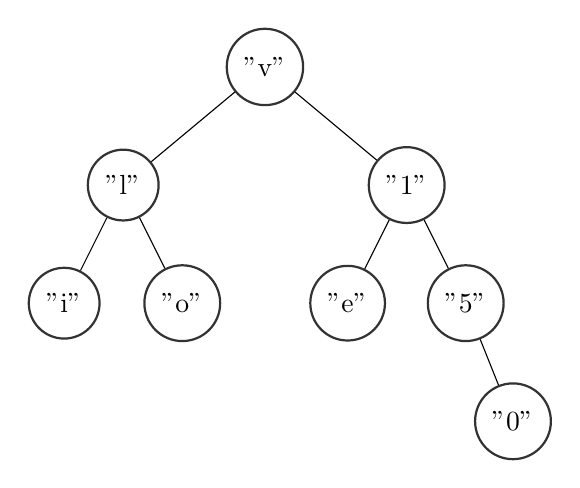
\begin{tikzpicture}
      [level distance=15mm,
      every node/.style={circle,inner sep=4pt, draw=black!80, thick},
      level 1/.style={sibling distance=36mm},
      level 2/.style={sibling distance=15mm},
      level 3/.style={sibling distance=12mm},
      ]
      \node {\code{"v"}}
        child {node {\code{"l"}}
          child {node {\code{"i"}}}
          child {node {\code{"o"}}}
        }
        child {node {\code{"1"}}
          child {node {\code{"e"}}}
          child {node {\code{"5"}}
            child[missing]
            child {node {\code{"0"}}}
          }
        };
      \end{tikzpicture}
  \end{center}

  \pause
  \vspace{\fill}

  \noteBox{}{ What the future looks like, now that we can put strings in trees.}
\end{frame}

\begin{frame}[fragile]
  \frametitle{Polymorphic Types, Polymorphic Functions}

  The fact that we can write these polymorphic functions on \code{list}s and
  \code{tree}s and the like is a \textit{result} of the fact that they are
  polymorphic types!

  \pause
  \vspace{\fill}

  We can write functions which respect the \textit{structure} of the type
  outside of the polymorphic parts, and are still able to do useful work.

  \pause
  \vspace{\fill}

  \begin{codeblock}
    fun count Empty = 0
      | count (Node (L, x, R)) = count L + 1 + count R

    fun safeValOf (default, NONE)   = default
      | safeValOf (default, SOME v) = v
  \end{codeblock}
\end{frame}

\begin{frame}[fragile]
  \frametitle{Generic Values}

  Through these declarations, it is possible to achieve polymorphic values that
  are not functions. While it may seem like type variables are only introduced
  by function arguments we do not know the type of, they are really introduced by
  any ambiguity in a type.

  \pause
  \vspace{\fill}

  For instance, what is the type of \code{[]}? We don't have enough information
  to constrain it either way, so the type is just \code{'a list}. This means that
  we could write the following code:

  \pause
  \vspace{\fill}

  \begin{codeblock}
    val l : 'a list = []
    val x : int list = 1 :: l
    val y : string list = "hi" :: l
  \end{codeblock}

  \pause
  The two instances of \code{l} are instantiated at \code{int list} and
  \code{string list}, respectively!
\end{frame}

\begin{frame}[fragile]
  \frametitle{Generic Types}

  It is now no longer true that each expression has only one type.

  \pause
  \vspace{\fill}

  For certain expressions like \code{fn x => x}, it could be
  interpreted to have multiple types, such as \code{int -> int}, or \code{'a -> 'a}.

  \pause
  \vspace{\fill}

  To explain away this ambiguity, we will revise our interest in types to be
  for the \term{most general type} for an expression.

  \pause
  \vspace{\fill}

  \defBox{ The \term{most general type} for an expression is the type that every
  other type for that expression is an instance of.}
\end{frame}

\begin{frame}[fragile]
  \frametitle{Type Instances}

  We spoke briefly on how different calls to \code{identity} were instances of
  the main declaration. We also define a concept of \term{instances} on types.

  \pause
  \vspace{\fill}

  \defBox{ A type \code{t1} is an \term{instance} of type \code{t2} if
  \code{t1} can be obtained from \code{t2} by substituting for some type variables.}

  \pause
  \vspace{\fill}

  So here are some examples:
  \begin{itemize}
    \item \code{int} is an instance of \code{'a}
    \item \code{int list} is an instance of \code{'a list}
    \item \code{int * int} is an instance of \code{'a * 'b}
    \item \code{int * bool} is an instance of \code{'a * 'b}
    \item \code{'b * 'c} is an instance of \code{'a}
    \item \code{'a list list} is an instance of \code{'a list}
  \end{itemize}
\end{frame}

\begin{frame}[fragile]
  \frametitle{Type Instances, Pictorially}

  \begin{center}
  \makebox[0.8\textwidth][c]{
    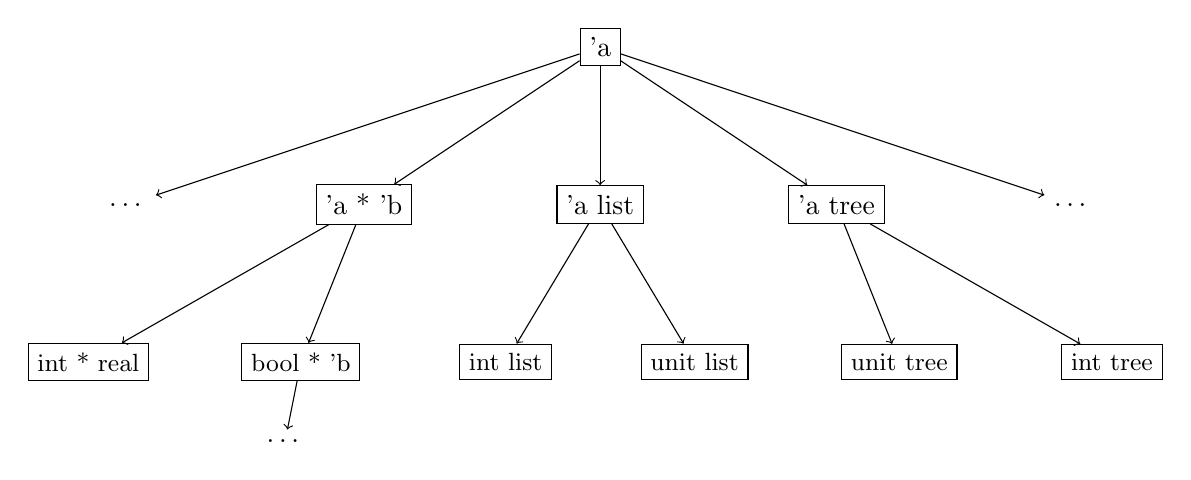
\begin{tikzpicture}
      \node[shape=rectangle,draw=black] (L1) at (-4.5,0) {\small \code{int * real}};

      \node[] (E2) at (-2,-1) {\textellipsis};
      \node[shape=rectangle,draw=black] (L2) at (-1.8,0) {\small \code{bool * 'b}};

      \node[shape=rectangle,draw=black] (L3) at (0.8,0) {\small \code{int list}};

      \node[shape=rectangle,draw=black] (L4) at (3.2,0) {\small \code{unit list}};

      \node[shape=rectangle,draw=black] (L5) at (5.8,0) {\small \code{unit tree}};

      \node[shape=rectangle,draw=black] (L6) at (8.5,0) {\small \code{int tree}};

      \node[] (EL) at (-4,2) {\textellipsis};
      \node[shape=rectangle,draw=black] (M1) at (-1,2) {\code{'a * 'b}};
      \node[shape=rectangle,draw=black] (M2) at (2,2) {\code{'a list}};
      \node[shape=rectangle,draw=black] (M3) at (5,2) {\code{'a tree}};
      \node[] (ER) at (8,2) {\textellipsis};

      \node[shape=rectangle,draw=black] (T) at (2,4) {\code{'a}};

      \draw[<-] (E2) -- (L2);

      \draw[<-] (L1) -- (M1);
      \draw[<-] (L2) -- (M1);
      \draw[<-] (L3) -- (M2);
      \draw[<-] (L4) -- (M2);
      \draw[<-] (L5) -- (M3);
      \draw[<-] (L6) -- (M3);

      \draw[<-] (EL) -- (T);
      \draw[<-] (M1) -- (T);
      \draw[<-] (M2) -- (T);
      \draw[<-] (M3) -- (T);
      \draw[<-] (ER) -- (T);
  \end{tikzpicture}
  }
  \end{center}

  \pause
  \vspace{\fill}

  Note that only the type \code{bool * 'b} has further instances, because
  it's the only one with a remaining type variable.

  \pause
  \vspace{\fill}

  We say that the rest of the types are \term{monomorphic}.
\end{frame}



\begin{frame}[fragile]
  \frametitle{Most General Types}

  So we see that the MGT of \code{length} is \code{'a list -> int},
  because while it can be typed as \code{int list -> int}, and
  \code{string list -> int}, among others, they are all just instances
  of the type \code{'a list -> int}.

  \pause
  \vspace{\fill}

  All parametric polymorphism is, is choosing instances of a most general
  type!

  \pause
  \vspace{\fill}

  \badBox{}{\, Be careful not to confuse being an \term{instance} of a type with
  a \term{most general type}. All types are instances of \code{'a}, but most
  expressions do not have MGT \code{'a}.
  }
\end{frame}

\begin{frame}[fragile]
  \frametitle{A Warning on Proofs}

  Beware the following common mistake on proofs!

  \pause
  \vspace{\fill}

  \thmBox{}{ \code{length (L @ R)} $\eeq$ \code{length L + length R} }

  \pause
  \vspace{\fill}

  When proving this claim on \code{length : 'a list -> int}, you might be tempted to
  write the following:

  \pause
  \vspace{\fill}

  We proceed by structural induction on \code{L : 'a list}.

  \vspace{\fill}

  \bcBox{\, \code{L = []}}

  \vspace{\fill}

  ...
\end{frame}

\begin{frame}[fragile]
  \frametitle{Type Quantification}

  This will get a point deduction! The quantification is incorrect.

  \pause
  \vspace{\fill}

  There is only one value of type \code{'a list}, so how can we possibly induct
  on it? To add another element would be to escape the type entirely, because
  that would specify the type of the list!

  \pause
  \vspace{\fill}

  The proper way to phrase the proof is:

  \pause
  \vspace{\fill}

  Let \code{t} be a type. We proceed by structural induction on \code{L : t list}.

  \vspace{\fill}

  ...

  \vspace{\fill}

  \ihBox{}{\, Case: \code{L = xs}, for some \code{xs : t list}. Assume ...}
  \isBox{}{Case: \code{L = x::xs}, for some \code{x : t}. Let's show ...}
\end{frame}

\begin{frame}[fragile]
  \frametitle{Parametric Types, Parametric Proofs}

  When proving a claim on values of a parametric type, you are essentially writing
  a proof for many types. To do this properly, you need to parameterize your proof
  by an arbitary type, and then proceed with the proof. This which will end up
  proving the claim for the parametric type.

  \pause
  \vspace{\fill}

  Another reason why the former proof doesn't work is that there are
  \textbf{no values of type \code{'a}}. This would entail a value which could
  be instantiated at any type, which obviously shouldn't exist!
\end{frame}

\begin{frame}[fragile]
  \frametitle{A Comment on Polymorphism}

  \tgs

  The conceptual takeaway is that a polymorphic type is a \textbf{family of types},
  parameterized by the input type. It is a \textbf{schema} that defines many other
  types.

  \pause
  \vspace{\fill}

  A function with a polymorphic type is a \textbf{family of functions}, all with
  the same implementation, but each with a different type depending on its usage.

  \pause
  \vspace{\fill}

  A proof on a function with a polymorphic type is a \textbf{family of proofs},
  one for each input type that the function could be instantiated at. We essentially
  are proving something for each function in the family of functions.
\end{frame}


\sectionSlide{4}{Polymorphic Sorting}

\begin{frame}[fragile]
  \frametitle{Generic Sorting}

  We've now addressed our over-reliance on \code{int}s in the context of functions like
  \code{length} and \code{identity}. Let's turn our attention towards a more classic problem,
  though.

  \pause
  \vspace{\fill}

  We previously discussed sorting, but only on integers! Let's abstract and try to create a
  \term{generic} sorting function. We'd like a function:

  \pause
  \vspace{\fill}

  \spec
    {sort}
    {'a list -> 'a list}
    {\code{true}}
    {\code{sort L} is a sorted permutation of \code{L}}

\end{frame}

\begin{frame}[fragile]
  \frametitle{On Sorting}

  ...But is that even a well-specified problem? What would it mean to have a function of
  type \code{'a list -> 'a list}?

  \pause
  \vspace{\fill}

  Recall that if we impose any constraints on what the type of the elements of the list are,
  then it will no longer generalize polymorphically. We have to somehow sort elements of a
  list without ever looking at what any given element is.

  \pause
  \vspace{\fill}

  It turns out, this function is impossible to write. Not in the least for the reason that
  "sorted" is a relative concept. We have an idea of a canonical sorting for integers --
  by magnitude. But what if we wanted to sort integers in reverse? Or modulo 12?
\end{frame}

\begin{frame}[fragile]
  \frametitle{Comparison Functions}

  All these notions involve what is called a \term{comparison function}.

  \pause
  \vspace{\fill}

  \defBox{}{ We say that a function \code{f : t * t -> order} is a \term{comparison function}
  if it is total, and defines a \term{total order}}

  \pause
  \vspace{\fill}

  \defBox{}{ A \term{total order} is a binary relation that essentially relates
  a bunch of things which can be ordered on a line. So
  a total order \code{f} should not have any cycles.}

  \pause
  \vspace{\fill}

  So we might define these comparison functions as:

  \begin{codeblock}
    val revIntCompare =
      fn (x, y) => case Int.compare (x, y) of
                     LESS => GREATER
                   | GREATER => LESS
                   | EQUAL => EQUAL
    val mod12Compare =
      fn (x, y) => Int.compare (x mod 12, y mod 12)
  \end{codeblock}
\end{frame}

\begin{frame}[fragile]
  \frametitle{The Meaning of Sorted}

  \rprs

  We can, relative to a comparison function \code{cmp : t * t -> order}, recursively
  define what it means for a list to be sorted with respect to that comparison
  function.

  \pause
  \vspace{\fill}

  \defBox{}{ We say that a list \code{L : t list} is \term{\code{cmp}-sorted}} if
  it has the following properties:

  \pause
  \begin{itemize}
    \item \code{L} $\eeq$ \code{[]}
    \item \code{L} $\eeq$ \code{[x]}
    \item \code{L} $\eeq$ \code{x::y::xs}, where \code{cmp (x, y)} $\eeq$
    \code{LESS} or \code{EQUAL}, and \code{y::xs} is \code{cmp}-sorted.
  \end{itemize}
\end{frame}

\begin{frame}[fragile]
  \frametitle{Sorting, Relatively}

  To be able to sort relatively, we will adjust the type of our \code{sort}
  function, slightly.

  \pause
  \vspace{\fill}

  Now, instead of being of type \code{'a list -> 'a list}, we will add a parameter
  to our \code{sort} function, which is a comparison function by which to sort.

  \pause
  \vspace{\fill}

  But wait, why can we take in a comparison function? Can functions be passed in as arguments?
\end{frame}

\begin{frame}[fragile]
  \frametitle{Functions are Values}

  This might come as a surprise\footnote{The same way that an annual tuition increase is a surprise.},
  but functions are values.

  \pause
  \vspace{\fill}

  We've seen it, by binding lambda expressions in \code{val} declarations, which
  is an equivalent form to the \code{fun} declarations we've been using so far.

  \pause
  \vspace{\fill}

  Another consequence of this is the fact that functions are \term{first-class citizens}.
  This means that they can be bound to values, passed into functions, and returned
  from functions, just like any other value.
\end{frame}

\begin{frame}[fragile]
  \frametitle{Functions are Values}

  We will discuss this more in-depth next lecture, but for this lecture, we will
  exploit the fact that functions can be passed in as arguments, to write our
  \code{sort} function in a way that it is \code{parameterized} by a comparison
  function.

  \pause
  \vspace{\fill}

  Essentially, what the \code{sort} function does, depends on what the comparison
  function is!
\end{frame}

\begin{frame}[fragile]
  \frametitle{Sorting, By Comparison}

  \spec
    {sort}
    {('a * 'a -> order) * 'a list -> 'a list}
    {\code{true}}
    {\code{sort (cmp, L)} is a \code{cmp}-sorted permutation of \code{L}}

  \pause
  \vspace{\fill}

  Let's implement this via our old definition of \code{msort}.
\end{frame}

\begin{frame}[fragile]
  \frametitle{\code{msort}, before}
  {\tiny
  \begin{codeblock}
    fun split [] = []
      | split [x] = [x]
      | split (x::y::xs) =
          let
            val (A, B) = split xs
          in
            (x::A, y::B)
          end

    fun merge ([], R) = R
      | merge (L, []) = L
      | merge (x::xs, y::ys) =
          if x < y then
            x :: merge (xs, y::ys)
          else
            y :: merge (x::xs, ys)

    fun msort [] = []
      | msort [x] = [x]
      | msort L =
          let
            val (A, B) = split L
          in
            merge (msort A, msort B)
          end
  \end{codeblock}
  }
\end{frame}


\begin{frame}[fragile]
  \frametitle{A Generic \code{msort}}
  {\tiny
  \begin{codeblock}
    fun split [] = []
      | split [x] = [x]
      | split (x::y::xs) =
          let
            val (A, B) = split xs
          in
            (x::A, y::B)
          end

    fun merge (`cmp`, ([], R)) = R
      | merge (`cmp`, (L, [])) = L
      | merge (`cmp`, (x::xs, y::ys)) =
          case `cmp (x, y)` of
            LESS => x :: merge (`cmp`, (xs, y::ys))
          | _ => y :: merge (`cmp`, (x::xs, ys))

    fun msort (`cmp`, []) = []
      | msort (`cmp`, [x]) = [x]
      | msort (`cmp`, L) =
          let
            val (A, B) = split L
          in
            merge (`cmp`, (msort (`cmp`, A), msort (`cmp`, B)))
          end
  \end{codeblock}
  }
\end{frame}

\begin{frame}[fragile]
  \frametitle{Finishing Off \code{sort}}


  All we did was pass the \code{cmp} function through, and then change a
  single place (where we used to do the integer comparison), instead using
  the provided comparison function. The code easily generalizes!

  \vspace{\fill}

  Now, we can define our \code{sort} function simply as:

  \pause
  \vspace{\fill}

  \begin{codeblock}
    fun sort (cmp : 'a * 'a -> order, L : 'a list) : 'a list = msort (cmp, L)
  \end{codeblock}

  \pause
  \vspace{\fill}

  Now we can sort generically! For instance, we have:
\end{frame}

\begin{frame}[fragile]
  \frametitle{\code{sort} Examples}

  \begin{itemize}
    \item \code{sort (Int.compare, [2, 3, 1])} $\hookrightarrow$ \code{[1, 2, 3]}
    \item \code{sort (String.compare, ["a", "ab", "b"])} $\hookrightarrow$ \code{["a", "b", "ab"]}
    \item \code{sort revIntCompare [1, 2, 3]} $\hookrightarrow$ \code{[3, 2, 1]}
  \end{itemize}
\end{frame}

% \begin{frame}[plain]
% 	\begin{center} Thank you! \end{center}

% 	\begin{center}
%     {\color{blue} \href{https://docs.google.com/forms/d/e/1FAIpQLSf9z0VuNTzebKdD29dw3k4sdp-SR8fQhxDoeBbZ7dSsMKtO5w/viewform?usp=sf_link}{Post-lecture survey:}} \\
%     \vspace{5pt}
%     \includegraphics[scale=0.035]{qr_june8}
%   \end{center}
% \end{frame}

\thankyou

\end{document}
